\chapter{Introduction}
\label{chap:intro}

\graphicspath{{Chapter1/figures/}}

\emph{Sensemaking} reflects how we make sense of the world so that we can take further actions in it~\cite{Snowden2005}. More specifically, sensemaking is described as a motivated and continuous effort to understand the relationships among people, places and events around us in order to act more effectively~\cite{Klein2006a}. It is the process of collecting, representing and organizing complex information sets based on a particular problem we are solving in such a way that can help us understand the problem better and make sense of it~\cite{Russell2008}. For example, intelligence analysts may need to examine thousands of reports to establish deep understanding of particular persons or organizations before identifying possible threats from them. In a more ordinary and everyday context such as selecting a smartwatch, a person may search for different models on the Internet, learn unfamiliar technical terminologies, and consider pros and cons between those identified models. To effectively make sense of the problem, people need to digest a large amount of data: a few tens of smartwach models, a few thousands of documents, or a much bigger scale. The data around the world has been produced more rapidly than ever before, with major sources including sensors, machine logs, public websites and social media. For a single day, 50 million photos are uploaded on Instagram, 500 million tweets are sent on Twitter, 3.5 billion searches are performed on Google and 200 billion emails are sent~\footnote{\url{http://www.internetlivestats.com/}}. This data deluge could help us find more relevant information to our problems; however, it also poses a huge challenge in making sense of such a vast amount of data.

\emph{Visualization} can help people solve problems more effectively through visual representations of datasets~\cite{Munzner2014}. They can display a large amount of data in a way that quickly reveals hidden patterns. Interaction allows people to further investigate the visualized data in more detail and explore the relationship between identified patterns. Automated techniques in information retrieval and data mining can help speed up the sensemaking process. For instance, named-entity recognition techniques~\cite{Nadeau2007} can automatically identify entities from text and classify them into predefined categories such as persons, organizations and locations. This automation saves analysts a considerable amount of time in their common tasks such as findings all reports mentioning a particular person. \emph{Visual analytics} combines such automated analysis techniques and interactive visualizations to effectively make sense of very large and complex datasets~\cite{Keim2010}.

Research in visual analytics focuses on helping people reveal hidden patterns in the data; however, sensemaking requires support beyond that. Analysts may connect individual patterns to explore the relationships between them, generate potential hypotheses explaining those relationships, and find ways to verify them. Unfortunately, people with limited capacity of working memory cannot hold all of these artifacts simultaneously. They may forget previous findings and relations between them, or remember but fail to retrieve the information needed. They may also forget how those findings were derived, making it more difficult to find similar information. Especially for long and interrupted analysis sessions with big datasets, people often get lost in the problem space: they are unable to examine their progresses, unable to synthesize their discoveries, and unable to decide the next step effectively.

\emph{Analytic provenance} has the potential to address these problems. It is a subfield of  visual analytics, focusing on understanding a user's reasoning process through the study of their interactions with the computer system that supports sensemaking~\cite{North2011}. Analytic provenance captures both the interactive data exploration process and the accompanied reasoning process during sensemaking~\cite{Xu2015}, releasing analysts from a burden of keeping track of their discoveries. Analytic provenance data can be categorized using a multiple semantic layer model~\cite{Gotz2009}. Low-level provenance can be captured automatically but contains little semantics. Higher level provenance contains richer semantics, thus could be more useful in sensemaking. However, it is much more challenging to capture and primarily has to be done manually. Visualizations of provenance data have been developed for different purposes including recall, replication, action recovery, collaborative communication, presentation and meta-analysis~\cite{Ragan2016}. Most of these visualizations provide post hoc applications of provenance or stop at recalling the process and revisiting past steps. They are not specifically designed to support the ongoing, iterative and dynamic sensemaking process.

\section{Research Problem and Approach}

The central research problem of this thesis is
\begin{center}
	\strong{How to design interactive visualizations of analytic provenance data \\for supporting sensemaking?}
\end{center}

To approach the research problem, we propose a cyclic process model, in which analytic provenance can be used to support sensemaking as illustrated in \autoref{fig:intro-workflow}. The process starts with a \emph{user} employing a \emph{sensemaking system} to solve a problem. The sensemaking system could be any computer-based applications, such as a simple visualization tool, a complex visual analytics system and a standard web browser. During the sensemaking process, both the performed low-level actions (e.g., visualization interaction such as sort, filter and zoom) and the produced high-level reasoning artifacts (e.g., findings, assumptions and hypotheses) are captured. They are referred as \emph{provenance data} in the figure. Then, this provenance data should be visualized in a way that can provide support back to the ongoing sensemaking process. In this model, the user can interact with both the sensemaking system and the \emph{provenance visualization} to solve his or her problem. The provenance visualization should be able to communicate with the sensemaking system to facilitate the interplay between the user and these two. Technically, it can be implemented directly in the sensemaking system or separately as a provenance-enabled plug-in.

\begin{figure}[!htb]
	\centering
	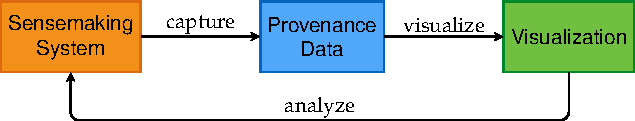
\includegraphics{workflow}
	\caption{A cyclic process model of supporting sensemaking through analytic provenance. While using a sensemaking system to solve a problem, the interaction and reasoning performed by the user are \emph{captured} and \emph{visualized} to provide \emph{support} back to the sensemaking process. The sensemaking system can be any computer-based applications such as visual analytics systems and web browsers. The two-way dash arrow indicates the communication between the provenance visualization and the sensemaking system to provide sensemaking support. As a result, the user can interact with both the sensemaking system and the provenance visualization to make sense of the problem.}
	\label{fig:intro-workflow}
\end{figure}

In this model, the provenance visualization takes input as the provenance data and output as the sensemaking support it provides. Therefore, in the scope of this thesis, it is essential to discuss what \textcm{\emph{data}} will be visualized and what \textch{\emph{tasks}} does the visualization aim to support.

\begin{enumerate}
	\item \textbf{What data will be visualized?}
	
	Both low-level actions (e.g., visualization interaction such as sort, filter and zoom) and high-level reasoning artifacts (e.g., findings, assumptions and hypotheses) are considered in this thesis. However, we do not examine bottom-level events such as mouse clicks and keystrokes because they contain very little semantics for supporting sensemaking~\cite{Gotz2009}. One inherent attribute of provenance data is \emph{time}, providing temporal information such as when an event happens. This attribute allows the review of the sensemaking process in chronological order.
	
	Additional relationship of the raw collected data could be useful for complex sensemaking tasks. This could come from an automated process such as topic modeling~\cite{Blei2003} to provide \emph{thematic information} for provenance data. This could also come from a manual assessment, in which a user can select relevant data items and assign \emph{pair-wise relations}. In a data abstraction language~\cite{Munzner2014}, the provenance data could contain an additional \emph{categorical} attribute or convert to a \emph{network} dataset, respectively.
	
	\item \textbf{What tasks does the visualization aim to support?}
	
	The characteristics of provenance data suggests the tasks it can support the users. The \emph{time} attribute of provenance data provides an opportunity to allow users to identify \emph{temporal} patterns and relationships in the sensemaking problem. This could enable users to recall their processes and reveal hidden storylines in the data. Timeline visualizations are often used to show such temporal relationship. However they are not specifically designed to support the iterative and dynamic nature of sensemaking. They are mainly used to present a known story instead of constructing a hidden one.
	
	As discussed earlier, grouping information can be added to help make sense of more complex temporal relationship. It allows users to examine storylines corresponding to individual groups and the interaction between them. However, existing visualizations are unable to effectively show both temporal and categorical information.
	
	After understanding how things happened, the next important step is	to explore the reason why they happened as they were. Understanding how users make sense of tasks is essential to build effective tools to support them. Can provenance data, especially low-level actions, help an analyst understand the \emph{rational} relationship of the sensemaking process?
	
	As discussed earlier, during sensemaking, users can enrich the provenance data by grouping and adding connections. Can the enriched provenance data help users explore more complex rational relationship of sensemaking? Does the benefit that users gain outweigh the overload that users involve in providing extra information richness?
\end{enumerate}

\autoref{fig:intro-work} summarizes the four research challenges described in this data -- task analysis.

\begin{figure}[!htb]
	\centering
	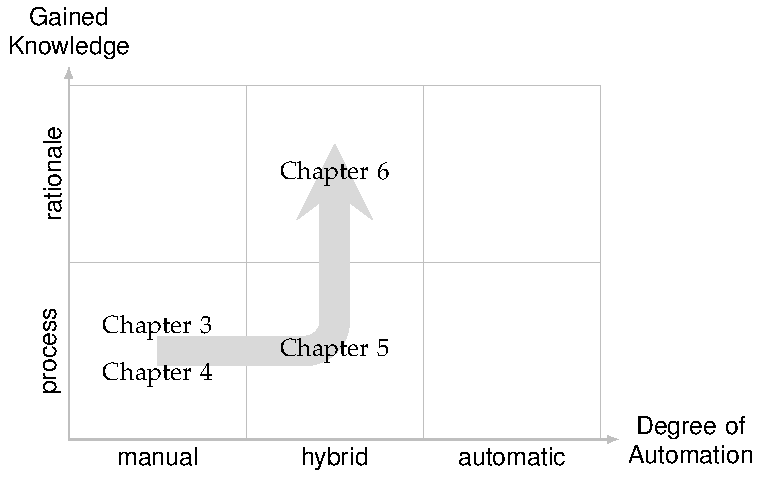
\includegraphics{work}
	\caption{Research problem split by \textcm{data} and \textch{task}. The horizontal axis represents different tasks and the vertical axis represents the complexity involved in the  task. The cells show the characteristics of data will be used to support the task.}
	\label{fig:intro-work}
\end{figure}

The research problem is broken into the following research questions based on the previous data -- task elaboration. They map to the four cells in \autoref{fig:intro-work}. For each question, we explain its context based on the sensemaking-support model described earlier: the sensemaking system, the user, the task and the provenance data. 

\begin{enumerate}
	\item How to design interactive visualizations of \textcm{time-oriented provenance data} 
	enabling users to explore \textch{temporal relationship of sensemaking}?
	
	The domain we target while addressing this research question is \emph{intelligence analysis} -- the original domain that set the foundation for visual analytics research~\cite{Thomas2005}. A common task for intelligence analysts is to examine thousands of reports to identify potential threats from particular persons or organizations. Many visual analytics have been designed to facilitate this analysis. These systems often allow users to take notes, recording the users' thought. We aim to augment these systems by a novel timeline visualization that enables users to identify temporal patterns and construct hidden stories from their annotations.
	
	\item How to design interactive visualizations that can utilize both \textcm{temporal and categorical provenance data} to reveal \textch{complex temporal relationship of sensemaking}?	
	
	This shares the same context with the previous research question. To the best of our knowledge, no existing visualization techniques is designed to show both temporal and categorical information effectively. Therefore, we also aim to design a general timeline visualization that can apply to other domains.
	
	\item How to design interactive visualizations that can exploit \textcm{time-oriented provenance data} to enable users to explore \textch{rational relationship of sensemaking}?
	
	To explore rational relationship of sensemaking, analysts often conduct a user study to observe the process, collect relevant data and analyze it. During the qualitative analysis, analysts may need to go through a lengthy process of transcribing the video recordings before coding the transcript with themes and building model based those themes. In this context, the sensemaking system mapped to \autoref{fig:intro-workflow} can be considered as a set of tools allowing the analysts to conduct a user study and analyze the collected data. We take a different approach to facilitate the transcription and coding steps. We capture analytic provenance while a user performs a sensemaking task and provide visualizations of the provenance data to enable the analyst explore the rational relationship of the user's sensemaking process. We focus only on browser-based sensemaking tasks. The provenance data could include information about visited web pages such as page URL, title and visit time.
	
	\item How to design interactive visualizations that can combine both \textcm{time-oriented provenance data and user-added relations} to enable users to explore \textch{complex rational relationship of sensemaking}?
	
	This research question targets a very common domain: browser-based online sensemaking. To make sense of everyday tasks such as selecting a camera, people often use standard web browsers -- simple sensemaking systems -- to search for different models and consider their strengths and weaknesses. The provenance data could include both automatically captured low-level actions as in the previous question and user-added relationship of the automatic capture such as by spatially grouping them or assigning pair-wise connections.
\end{enumerate}

We take a user-centered design approach in seeking solutions to all the research questions. For each question, we elicit the design requirements by conducting a user study and/or drawing from the literature. Visual encoding and interaction are designed to meet those requirements, and the designs are implemented into a working prototype. Finally, an empirical study is conducted to explore how the tool is used by target audience and check whether it provides the intended support. 

\section{Thesis Contributions}
Toward the overall goal of supporting users in their sensemaking processes through the visualizations of provenance data, this thesis contributes:

\begin{itemize}
	\item A timeline visualization technique -- \emph{\textcb{SchemaLine}} -- that enables users to examine information in chronological order, identify temporal patterns and construct narratives from relevant user annotations. SchemaLine produces a compact but aesthetically pleasing layout and provides a set of fluid interactions allowing users to perform various sensemaking activities described in the Data--Frame model~\cite{Klein2003}. This is to address Research Question 1, and the work is published as 
	
	\textbf{P. H. Nguyen}, K. Xu, R. Walker, and B. L. W. Wong. SchemaLine: Timeline Visualization for Sensemaking. In \textit{International Conference on Information Visualization}, pages 225--233. IEEE, jul 2014.
	
	\item A timeline visualization technique -- \emph{\textcb{TimeSets}} -- that enables users to explore complex temporal relationship by effectively representing both temporal and categorical provenance data. TimeSets visually groups data items that share the same group but still preserves their temporal order. It color codes the backgrounds of the entire groups to distinguish them and uses colored gradient backgrounds for the intersections among those groups. It also adjusts the level of details of each data item dynamically to accommodate more items within a given display estate. This is to address Research Question 2, and the work is published as  
	
	\textbf{P. H. Nguyen}, K. Xu, R. Walker, and B. L. W. Wong. TimeSets: Timeline visualization with set relations. \textit{Information Visualization}, 15(3):253--269, jul 2016. 
	
	and for the VAST Challenge case study as
	
	\item K. Xu, \textbf{P. H. Nguyen}, and B. Fields. Visual analysis of streaming data with SAVI and SenseMAP. In \textit{IEEE Conference on Visual Analytics Science and Technology}, pages 389--390. IEEE, oct 2014.
	 
	\item A visual sensemaking tool -- \emph{\textcb{SensePath}} -- that enables analysts to explore rational relationship of the sensemaking process. Qualitative research methods are often used in understanding rational relationship of sensemaking. This is a manual and time-consuming process: researchers collect observation data, transcribe screen capture videos and think-aloud recordings, identify recurring patterns, and eventually abstract the sensemaking process into a general model. SensePath offers an alternative and possibly faster approach in performing transcription and coding. In stead of having to transcribe the video, SensePath automatically captures and detects participant's sensemaking actions, and provides multi-linked visualizations to support further analysis. It visualizes provenance data in a timeline that enables researchers to quickly gain an overview of the sensemaking process and identify recurring sensemaking patterns. It also links with a screen capture video to allow researchers to examine  additional context when necessary. Finally, to enable researchers to continue working on later stages of analysis using their normal workflow, SensePath exports its coded transcript in a common format that can be used by other popular qualitative data analysis software packages. This is to address Research Question 3, and the work is published as
	
	\textbf{P. H. Nguyen}, K. Xu, A. Wheat, B. L. W. Wong, S. Attfield, and B. Fields. SensePath: Understanding the Sensemaking Process through Analytic Provenance. \textit{IEEE Transactions on Visualization and Computer Graphics}, 22(1):41--50, jan 2016. 
	
	\item A visual sensemaking tool -- \emph{\textcb{SenseMap}} -- that enables users to explore complex rational relationship of sensemaking. It automatically captures and detects sensemaking actions and relationships between these actions before visualizing both of them in a branching history tree. This allows users to examine the rational relationship between the actions they performed and potentially helps them remind of what have been done earlier. SenseMap offers users to assign additional meaning to the automatically collected data by spatially grouping actions or adding rational links between them, in order to help explain complex relationship. Finally, SenseMap allows users to communicate their analysis results at different levels of granularity including a big picture of user-organized findings, a more detailed analysis process and raw provenance data captured. This is to address Research Question 4, and the work is published as 

	\textbf{P. H. Nguyen}, K. Xu, A. Bardill, S. Betul, K. Herd, and B. L. W. Wong. SenseMap: Supporting Browser-based Online Sensemaking through Analytic Provenance. In \textit{IEEE Conference on Visual Analytics Science and Technology}, 2016.
\end{itemize}

Besides the main contributions described in this thesis, I also coauthored two other publications, contributing my knowledge in provenance for sensemaking.

\begin{itemize}
	\item I contributed to the discussion and the design of a framework for provenance in human terrain analysis, and the work was published as
	
	R. Walker, A. Slingsby, J. Dykes, K. Xu, J. Wood, \textbf{P. H. Nguyen}, D. Stephens, B. L. W. Wong, and Y. Zheng. An extensible framework for provenance in human terrain visual analytics. \textit{IEEE Transactions on Visualization and Computer Graphics}, 19(12):2139--2148, dec 2013.
	
	\item I contributed to the organization of a IEEE VIS workshop on provenance for sensemaking. The discussion at the workshop was published as
	
	K. Xu, S. Attfield, T. J. Jankun-Kelly, A. Wheat, \textbf{P. H. Nguyen}, and N. Selvaraj. Analytic provenance for sensemaking: a research agenda. IEEE Computer Graphics and Applications, 35(3):56--64, jan 2015.	
\end{itemize}

\section{Thesis Outline} 
The remainder of this thesis is organized as follows.

First, \autoref{chap:review} reviews the core work related to sensemaking, analytic provenance and visualization. Then, it emphasizes on the visualization of provenance data for supporting sensemaking. At the end, this chapter presents visualization techniques of general time-oriented and network data because these types of data have similar characteristics as provenance data.

\autoref{chap:schemaline} discusses the SchemaLine timeline visualization of user annotations enabling the users to explore temporal relationship of sensemaking -- addressing Research Question 1.

\autoref{chap:timesets} extends \autoref{chap:schemaline} to present the TimeSets visualization technique that can effectively show both temporal and categorical provenance data in order to reveal complex temporal relationship of sensemaking -- addressing Research Question 2.

\autoref{chap:sensepath} discusses the SensePath visualization tool that can exploit time-oriented provenance data, enabling users to explore rational relationship of sensemaking -- addressing Research Question 3.

\autoref{chap:sensemap} describes the SenseMap visualization tool that can utilize both temporal and relational provenance data enabling users to explore complex rational relationship of sensemaking -- addressing Research Question 4.

Finally, \autoref{chap:conclusion} concludes the thesis with a discussion on its contributions and future research directions triggered from this work.